\documentclass[11pt,letterpaper]{article}
\usepackage[T1]{fontenc}
\usepackage[utf8]{inputenc}
\usepackage[spanish,es-nodecimaldot]{babel}
\usepackage{lmodern,graphicx,tabularx,booktabs,array,caption,fancyhdr,titlesec}
\usepackage[table]{xcolor}
\usepackage[letterpaper,left=24mm,right=24mm,top=24mm,bottom=22mm,headheight=15pt]{geometry}
\usepackage[hidelinks]{hyperref}
\definecolor{vino}{HTML}{7A1F2B}\definecolor{titulo}{HTML}{551620}\definecolor{rosa}{HTML}{F5EDEE}
\renewcommand{\familydefault}{\sfdefault}
\titleformat{\section}{\Large\bfseries\color{titulo}}{\thesection.}{.4em}{}
\titleformat{\subsection}{\large\bfseries\color{vino}}{\thesubsection.}{.4em}{}
\titlespacing*{\subsection}{0pt}{11pt}{3pt}
\setlength{\parindent}{0pt}\setlength{\parskip}{5pt}
\pagestyle{fancy}\fancyhf{}\fancyhead[R]{\small\color{vino}UNSAAC · Ingeniería Informática y de Sistemas}
\fancyfoot[L]{\small Desarrollo de Software II · IF616BIN}\fancyfoot[R]{\small Sesión 2 · Página \thepage}
\renewcommand{\headrulewidth}{.4pt}
\renewcommand{\arraystretch}{1.28}
\newcommand{\tabla}[2]{\par\smallskip\begin{tabularx}{\linewidth}{@{}>{\bfseries\color{vino}}p{.28\linewidth}X@{}}\toprule\rowcolor{rosa}#1\\\midrule #2\bottomrule\end{tabularx}\par}
\newcommand{\ruta}[1]{\nolinkurl{#1}}
\newcommand{\foto}[3]{\begin{minipage}[t]{.48\linewidth}\centering\includegraphics[height=#1,keepaspectratio]{evidencias/#2}\captionof{figure}{#3}\end{minipage}}
\captionsetup{font=small,labelfont=bf,hypcap=false}
\begin{document}
\begin{titlepage}\centering
{\color{vino}\bfseries UNIVERSIDAD NACIONAL DE SAN ANTONIO ABAD DEL CUSCO\\[4pt]
\small FACULTAD DE INGENIERÍA ELÉCTRICA, ELECTRÓNICA, INFORMÁTICA Y MECÁNICA\\
ESCUELA PROFESIONAL DE INGENIERÍA INFORMÁTICA Y DE SISTEMAS\par}
\vspace{5mm}

\includegraphics[height=2cm]{evidencias/insignia.png}\hspace{1cm}
\includegraphics[height=2cm]{evidencias/escuela.jpg}\par
\vfill
{\LARGE\bfseries\color{titulo} DESARROLLO DE SOFTWARE II\par}
Código IF616BIN — Semestre Académico 2026-II\par
\vspace{6mm}
{\large\bfseries\color{titulo} INFORME DE PRÁCTICA — SESIÓN 2\par}
{\Large\bfseries\color{titulo} Informe de los cuatro retos\\Wallet UNSAAC\par}
\vspace{4mm}
Segunda Unidad Didáctica · Integración con servicios web y APIs\\
Sesión 2 · miércoles 11 de noviembre de 2026\par
\vfill
\raggedright
\tabla{Asignatura & Desarrollo de Software II}{Código & IF616BIN\\Unidad / sesión & Unidad II — Sesión 2\\Producto & Primer flujo BLoC y pruebas unitarias en Wallet UNSAAC\\Evaluación & Entregable D1, 8\,\% · Rúbrica analítica de 20 puntos\\Modalidad & Individual\\Docente & Mtro. Ing. Yover Collantes Valer\\Estudiante & Axel Barnaby Aranibar Rojas · 220547\\}
\vfill\centering Escuela Profesional de Ingeniería Informática y de Sistemas\\Semestre Académico 2026-II · Cusco, Perú
\end{titlepage}
\section{Datos generales}
\tabla{Campo & Información}{Nombre y apellidos & Axel Barnaby Aranibar Rojas\\Código de estudiante & 220547\\Escuela profesional & Ingeniería Informática y de Sistemas\\Asignatura & Desarrollo de Software II (IF616BIN)\\Unidad / sesión & Unidad II — Sesión 2 · 11 de noviembre de 2026\\Docente & Mtro. Ing. Yover Collantes Valer\\Repositorio de origen & \url{https://github.com/axelIn06/wallet-unsaac-aranibar-rojas}\\Revisión de la aplicación & Rama \texttt{sesion-02}, commit \texttt{aa09a28}\\Fecha del informe & 24 de noviembre de 2026\\Retos entregados & Edición, guardado visible, error con reintento y filtro por tipo\\}
\section{Resumen del trabajo}
La práctica amplía Wallet UNSAAC con un historial de movimientos que permite registrar ingresos y egresos, corregir un importe, eliminar una operación y vaciar la lista previa confirmación. El usuario también puede consultar un solo tipo de movimiento mientras la tarjeta superior conserva los totales de la billetera. Cada acción genera un evento que procesa el bloc de movimientos. El repositorio en memoria devuelve un resumen nuevo y el dominio calcula el saldo en céntimos.

Los cuatro retos cubren situaciones observables. Una corrección conserva el identificador y la posición del movimiento. Durante un alta se mantiene la lista anterior hasta que termina la escritura. Si el repositorio falla, la pantalla conserva el último resumen disponible y ofrece una recarga. Al seleccionar un filtro cambia el historial visible y se conserva la selección al registrar otra operación. La verificación combinó análisis estático, compilación para Android y 36 pruebas automatizadas. Las pruebas de interfaz ejercitaron el formulario y el reintento con el mismo árbol de widgets que utiliza la aplicación.

\textbf{Palabras clave.} Flutter, BLoC, repositorio, inmutabilidad, pruebas unitarias.
\newpage
\begingroup\small\renewcommand{\arraystretch}{1.13}\section{Entorno y verificaciones}
\subsection{Versiones utilizadas}
\tabla{Herramienta & Versión o configuración}{Flutter / Dart & 3.41.6 estable / 3.11.4\\Android & AVD Medium Phone API 36.1, arquitectura arm64\\Sistema & macOS 27.0\\Firebase & SDK integrado. La práctica utiliza el repositorio local.\\Dependencias del flujo & \texttt{flutter\_bloc} 9.1.1 y \texttt{bloc\_test} 10.0.0. Las versiones resueltas se conservan en \ruta{pubspec.lock}.\\}
\subsection{Comandos ejecutados}
\tabla{Comando & Resultado}{\ruta{flutter pub get --offline} & Resolución desde la caché del equipo.\\\ruta{flutter analyze --no-pub} & Análisis sin observaciones.\\\ruta{flutter test --no-pub} & 15 pruebas en la base heredada y 36 en la entrega final.\\\ruta{flutter build apk --debug} & Gradle generó \ruta{app-debug.apk}.\\\ruta{flutter run} & Instalación y arranque en el emulador Android.\\}
\begin{center}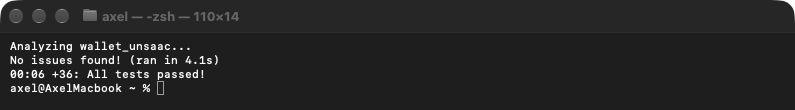
\includegraphics[width=.9\linewidth]{evidencias/consola.png}
\captionof{figure}{Ventana de Terminal con la salida del analizador y la última línea de la suite. Los registros completos se conservan en \ruta{evidencias/sesion-02/} del proyecto.}\end{center}
\subsection{Estructura del repositorio}
\texttt{domain/} define los movimientos, el resumen y las operaciones disponibles. \texttt{data/} implementa esas operaciones sobre una lista privada. \texttt{presentation/} contiene el bloc, los eventos, los estados y las pantallas. Las tres carpetas se encuentran en \ruta{lib/features/wallet/}. \ruta{lib/app.dart} proporciona el repositorio al bloc y \ruta{test/} contiene las pruebas.
\newpage
\endgroup\section{Reto 1 — Edición de un movimiento}
\subsection{Objetivo y alcance}
Corregir el título y el monto de un movimiento ya registrado. El historial conserva el identificador, el orden y la cantidad de filas.
\subsection{Diseño de la solución}
\tabla{Elemento & Decisión y justificación}{Identidad & \ruta{Movement.copyWith} construye una entidad con el mismo ID y admite cambios de título, categoría, monto, tipo o fecha.\\Edición & El formulario precarga título e importe. El repositorio busca el ID y reemplaza la fila en su índice.\\Precisión & El formulario separa soles y céntimos a partir del texto. El dominio suma cantidades enteras.\\}
\subsection{Implementación}
\ruta{presentation/pages/movement_editor.dart} valida título e importe y devuelve el movimiento corregido. \ruta{presentation/bloc/movements_bloc.dart} recibe \texttt{MovementUpdated}. El repositorio localiza la fila con \texttt{indexWhere} y aplica el reemplazo:
\begin{verbatim}
_items[index] = movement;
return WalletSummary(_items);
\end{verbatim}
Un ID ausente produce un error observable. Esta decisión impide registrar como alta una edición sobre un elemento que ya fue eliminado.
\subsection{Pruebas ejecutadas}
\tabla{Prueba & Resultado observado}{Prueba del bloc & Un ingreso de S/ 100,00 y un gasto corregido de S/ 5,00 a S/ 8,50 dejan S/ 91,50. El gasto ocupa la segunda fila con el mismo ID.\\Prueba del formulario & El menú permite cambiar el título a «Internet corregido» y el gasto a S/ 80,00. Permanecen siete filas y el saldo sube a S/ 1\,284,50.\\}
\newpage
\subsection{Evidencias}
\noindent\foto{10.5cm}{editar.png}{El formulario recupera el título y los S/ 89,90 originales.}\hfill
\foto{10.5cm}{editado.png}{La corrección a S/ 80,00 aumenta el saldo en S/ 9,90. El movimiento sigue primero.}
\subsection{Dificultades y decisiones}
El importe se muestra en soles y el dominio trabaja en céntimos. Se aceptaron punto y coma decimal y se limitó la parte fraccionaria a dos dígitos. La prueba de interfaz introduce \texttt{80,00} para verificar esa conversión.
\subsection{Autoevaluación}
\tabla{Criterio & Evidencia}{ID y posición estables & La prueba del bloc compara la lista completa y el ID de la última fila.\\Saldo y cantidad & La prueba del formulario comprueba el nuevo saldo y siete movimientos.\\Edición accesible & Cada menú lleva la etiqueta «Acciones de» seguida del título del movimiento.\\}
\newpage
\section{Reto 2 — Guardado visible con copyWith}
\subsection{Objetivo y alcance}
Mostrar que se está registrando una operación durante el intervalo entre el toque y la respuesta del repositorio.
\subsection{Diseño de la solución}
\tabla{Elemento & Decisión y justificación}{Estado & \ruta{MovementsReady} contiene el resumen, el filtro y la bandera \texttt{isSaving}, inicialmente falsa.\\Igualdad & Los tres campos participan en \texttt{props}. Así, activar el indicador produce un cambio observable incluso con los mismos movimientos.\\Interfaz & Un selector observa la bandera y muestra una barra lineal encima de las acciones.\\}
\subsection{Implementación}
Al recibir \texttt{MovementAdded}, el bloc conserva una referencia al último resumen visible. Antes de esperar la escritura, emite una copia:
\begin{verbatim}
emit(previous.copyWith(isSaving: true));
\end{verbatim}
Al completar el alta, construye otro \texttt{MovementsReady} con el resumen devuelto. La bandera recupera su valor predeterminado. La cola del bloc ordena las operaciones para que una respuesta anterior no sobrescriba el resultado de una posterior.
\subsection{Pruebas ejecutadas}
\tabla{Prueba & Resultado observado}{Secuencia del alta & La primera emisión conserva la lista original y activa el guardado. La segunda contiene el elemento añadido y desactiva la bandera.\\Igualdad & Una copia sin cambios es igual al original. Cambiar solo \texttt{isSaving} produce un estado distinto.\\Escrituras consecutivas & Un alta seguida de una baja conserva ambos efectos y el saldo coincide con la lista final.\\}
\newpage
\subsection{Evidencias}
\noindent\foto{10.5cm}{guardando.png}{Alta en curso. La barra bajo la tarjeta acompaña el saldo anterior y las siete filas.}\hfill
\foto{10.5cm}{guardado.png}{Alta completada. Aparece «Ingreso de práctica» por S/ 10,00, con ocho movimientos.}
\subsection{Dificultades y decisiones}
Una captura tomada después de estabilizar toda la interfaz solo muestra el resultado final. Para observar la transición se capturó el widget a los 220 milisegundos de iniciar el alta, dentro de la latencia simulada de 650 milisegundos.
\subsection{Autoevaluación}
\tabla{Criterio & Evidencia}{Continuidad de la lista & La captura de guardado conserva los datos previos.\\Fin de la escritura & El saldo pasa de S/ 1\,284,50 a S/ 1\,294,50 en el recorrido ilustrado.\\Secuencia e inmutabilidad & La prueba del bloc compara ambas emisiones y la prueba de estado verifica la igualdad de copias.\\}
\newpage
\section{Reto 3 — Error visible y reintento}
\subsection{Objetivo y alcance}
Informar de un fallo y permitir que el usuario recargue el historial. Si el error ocurre durante una escritura, la pantalla conserva el último resumen confirmado.
\subsection{Diseño de la solución}
\tabla{Situación & Respuesta de la interfaz}{Fallo inicial & Al faltar un resumen previo, la pantalla presenta el mensaje y una acción de reintento.\\Fallo de escritura & El estado \texttt{MovementsFailure} conserva el resumen anterior. La lista sigue disponible y un \texttt{SnackBar} identifica la operación fallida.\\Reintento & El botón envía \texttt{MovementsStarted}. La recarga consulta los datos actuales antes de que el usuario decida repetir el alta.\\}
\subsection{Implementación}
En \ruta{wallet_home_page.dart}, el listener de \texttt{BlocConsumer} restringe los avisos a nuevos fallos:
\begin{verbatim}
listenWhen: (previous, current) =>
    current is MovementsFailure && current != previous,
\end{verbatim}
El constructor de \texttt{WalletApp} recibe un \texttt{WalletRepository}. La prueba inyecta una implementación local cuyo primer intento de alta falla. Conservar el último resumen impide que una escritura rechazada altere el dinero mostrado.
\subsection{Pruebas ejecutadas}
\tabla{Prueba & Resultado observado}{Fallo de alta & Aparece un único aviso; permanecen «Plan de internet» y el saldo de S/ 1\,274,60 en la semilla de prueba.\\Reintento desde el aviso & La prueba toca la acción, verifica dos consultas acumuladas al repositorio y vuelve a encontrar los siete movimientos.\\Fallo inicial & La primera consulta falla y el reintento recupera el resumen. La prueba utiliza datos locales.\\}
\newpage
\subsection{Evidencias}
\noindent\foto{10.5cm}{error.png}{Fallo de alta después de la edición. Abajo aparece «Reintentar» y el saldo sigue en S/ 1\,284,50.}\hfill
\foto{10.5cm}{inicio_widget.png}{Referencia anterior a la edición. La prueba independiente arranca con siete movimientos y S/ 1\,274,60.}
\subsection{Dificultades y decisiones}
Un mensaje transitorio podía volver a aparecer al reconstruir la pantalla. El listener comprueba que cambió el estado y el constructor usa el último resumen confirmado. Para reproducir el caso en Android se ejecuta \ruta{flutter run --dart-define=DEMO_FALLO_ALTA=true} y se pulsa «Ingreso».
\subsection{Autoevaluación}
\tabla{Criterio & Evidencia}{Mensaje visible & La prueba busca exactamente un \texttt{SnackBar} con el texto del fallo.\\Contexto conservado & El saldo y la lista siguen visibles antes de pulsar «Reintentar».\\Recuperación sin red & El contador del repositorio inyectado demuestra que se realiza otra consulta.\\}
\newpage
\section{Reto 4 — Filtro por tipo con BlocSelector}
\subsection{Objetivo y alcance}
Consultar todos los movimientos, solo los ingresos o solo los egresos, manteniendo un saldo general que represente toda la billetera.
\subsection{Diseño de la solución}
\tabla{Elemento & Decisión y justificación}{Selección & \texttt{MovementFilter} pertenece al estado de presentación. \texttt{visibleMovements} devuelve los elementos del tipo seleccionado.\\Tarjeta de saldo & Su \texttt{BlocSelector} observa únicamente \texttt{WalletSummary}. Un cambio de filtro conserva ese valor.\\Persistencia del filtro & El bloc lleva el filtro anterior al estado que emite después de un alta, edición o baja.\\}
\subsection{Implementación}
El control segmentado emite \texttt{MovementsFilterChanged}. Con un estado listo, el manejador aplica:
\begin{verbatim}
emit(current.copyWith(filter: event.filter));
\end{verbatim}
El resumen sigue conteniendo ingresos y egresos. La lista obtiene su proyección de \texttt{visibleMovements} y muestra el número de filas visibles. El selector de la lista ignora los cambios que solo afectan al indicador de guardado.
\subsection{Pruebas ejecutadas}
\tabla{Selección & Resultado con S/ 100,00 de ingreso y S/ 5,00 de egreso}{Ingresos & Solo aparece la beca. El saldo continúa en S/ 95,00.\\Egresos & Solo aparece el pasaje. El saldo continúa en S/ 95,00.\\Todos & Se recuperan ambas filas en el orden original y el mismo objeto de resumen.\\Alta bajo filtro & Al agregar un egreso bajo el filtro de ingresos, la lista sigue mostrando la beca y el saldo general se actualiza.\\}
\newpage
\subsection{Evidencias}
\noindent\foto{10.5cm}{guardado.png}{Con «Todos», la tarjeta resume ocho movimientos y muestra S/ 1\,294,50.}\hfill
\foto{10.5cm}{filtro.png}{Con «Egresos», quedan cuatro filas. El saldo y ambos totales se mantienen.}
\subsection{Dificultades y decisiones}
Si la tarjeta recibiera el subconjunto filtrado, el usuario vería un saldo diferente al cambiar de pestaña. La selección se limita a la lista. Las tres pruebas independientes comprueban tanto el contenido visible como la identidad del resumen.
\subsection{Autoevaluación}
\tabla{Criterio & Evidencia}{Tres filtros operativos & Un caso independiente por valor de \texttt{MovementFilter}.\\Saldo constante & Las dos figuras mantienen S/ 1\,294,50 con cantidades de filas distintas.\\Filtro tras escritura & La prueba «Conserva el filtro al agregar» verifica la lista y el nuevo saldo.\\}
\newpage
\section{Conclusiones y aprendizajes}
\begin{enumerate}
\item Mantener el ID y sustituir el movimiento en su índice permite corregir un gasto sin alterar la posición. El caso del plan de internet disminuyó el egreso en S/ 9,90 y aumentó el saldo por el mismo importe.
\item Conservar el último resumen confirmado permite distinguir una escritura pendiente de una ya aceptada. La prueba del alta observa dos emisiones y la del fallo comprueba que el saldo previo sigue en pantalla.
\item El filtro pertenece a la vista del historial. Seleccionar únicamente el resumen para la tarjeta mantiene visibles los totales de la billetera al pasar de ocho movimientos a cuatro egresos.
\end{enumerate}
\section{Declaración de originalidad y uso de herramientas de IA}
Se utilizó OpenAI Codex para adaptar el proyecto de la sesión 1, generar y revisar código y pruebas, operar el emulador, capturar evidencias y redactar el informe en LaTeX. Los resultados consignados proceden de ejecuciones locales. La revisión personal del contenido y la firma corresponden al estudiante.
\medskip

Firma del estudiante: \rule{6cm}{.4pt}\hfill Fecha: \rule{2.7cm}{.4pt}
\section{Referencias}
Google. (s. f.). \textit{Get started with Firebase in your Flutter project}. Firebase. \url{https://firebase.google.com/docs/flutter/setup}

Universidad Nacional de San Antonio Abad del Cusco. (2026a). \textit{Guía de aplicación — Sesión 2: Primer flujo BLoC y pruebas unitarias} [Guía de práctica]. Desarrollo de Software II.

Universidad Nacional de San Antonio Abad del Cusco. (2026b). \textit{Sesión 2: Flujo BLoC y pruebas} [Material de la Unidad II]. Desarrollo de Software II.

Universidad Nacional de San Antonio Abad del Cusco. (2026c). \textit{Plantilla de informe — Sesión 1: Informe de los cuatro retos} [Plantilla de entrega]. Desarrollo de Software II.
\newpage
\section*{Anexo A. Lista de verificación de entrega}
\tabla{Verificación & Estado}{Compilación y análisis & Verificados en Android y con \texttt{flutter analyze}.\\Pruebas & 36 aprobadas. Registro completo en \ruta{evidencias/sesion-02/test.txt}.\\Cuatro retos & Implementados. Pruebas y evidencias en las secciones 4 a 7.\\Plantilla & Numeración de apartados, portada, referencias y autoevaluación adaptadas a la sesión 2.\\Firebase & Modo local permitido para D1. El README explica la vinculación con el proyecto Android del estudiante.\\Firma y aula virtual & Pendientes de revisión y presentación por el estudiante.\\}
\begin{center}
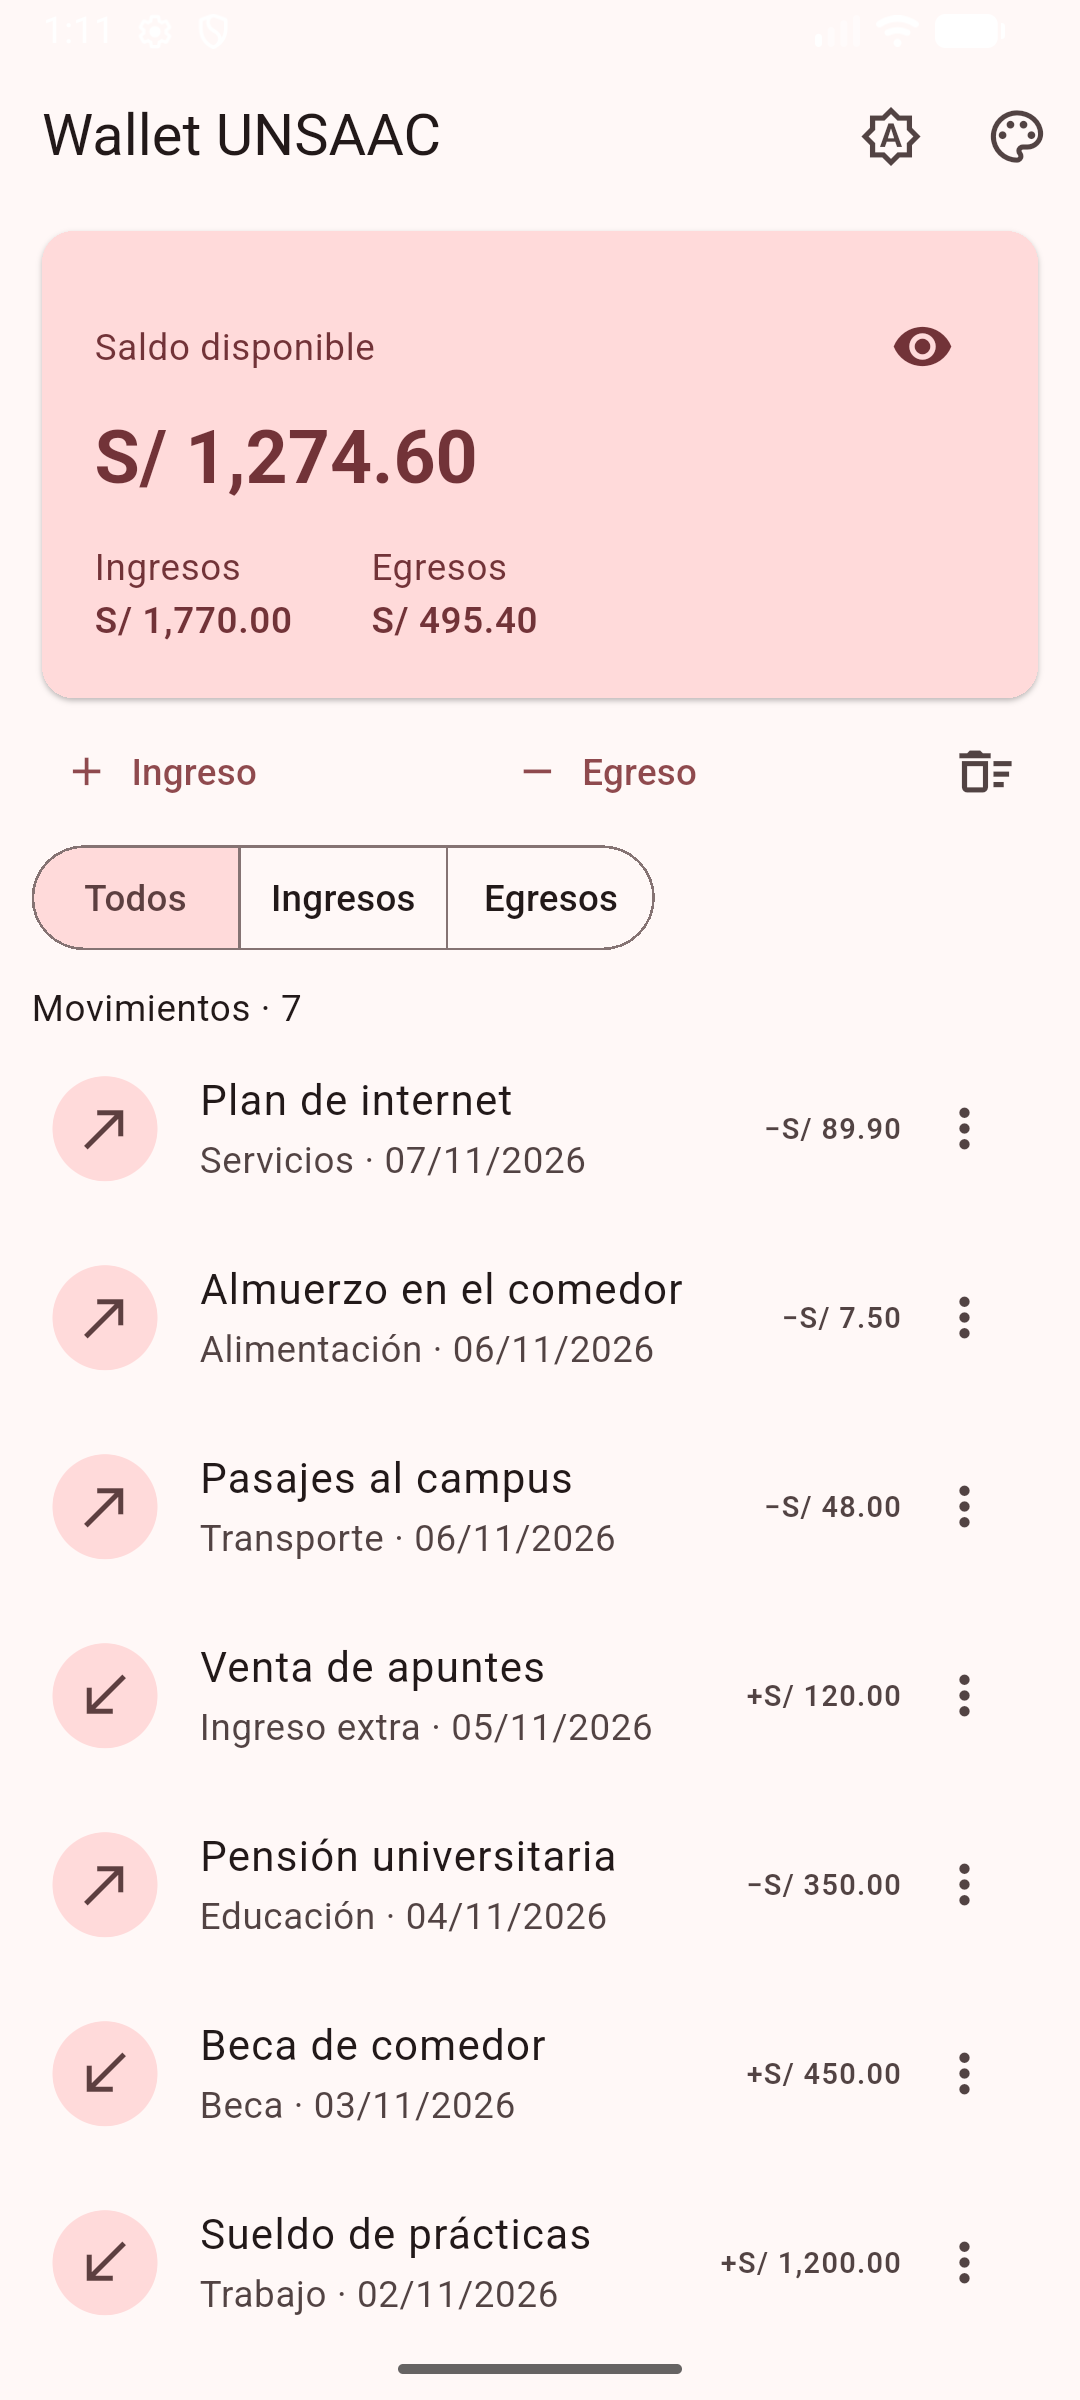
\includegraphics[height=9.6cm]{evidencias/android.png}
\captionof{figure}{Ejecución en el emulador Android. El saldo inicial de S/ 1\,274,60 resulta de S/ 1\,770,00 de ingresos menos S/ 495,40 de egresos.}
\end{center}
{\small La figura del anexo procede del emulador. Las figuras de los retos se capturaron directamente del árbol de widgets de \texttt{WalletApp} durante un recorrido reproducible con el repositorio local.}
\end{document}
